%----------------------------------------------------------------------------------------
\chapter{Esempi Trasposti in Collektive}
\label{chap:trasposizione}
%----------------------------------------------------------------------------------------

In questo capitolo si presenta la trasposizione di una selezione di programmi aggregati, originariamente sviluppati in Proto (\Cref{chap:mitproto}), nel linguaggio Collektive (\Cref{chap:collektive}).
%
Per ciascun esempio viene illustrato il codice sorgente originale, una descrizione dettagliata del funzionamento, la relativa implementazione in Collektive e le immagini delle simulazioni realizzate.

Gli esempi selezionati comprendono: calcolo della media locale (\Cref{sec:localaverage}), verifica dell’appartenenza a una regione circolare (\Cref{sec:incircle}), identificazione dei dispositivi lungo un anello (\Cref{sec:ring}), diffusione della temperatura (\Cref{sec:temperature}), navigazione lungo la discesa del gradiente (\Cref{sec:navgrad}), partizionamento di Voronoi (\Cref{sec:voronoi}), connessione lungo l’albero dei cammini minimi (\Cref{sec:wire}), tracciamento di un dispositivo (\Cref{sec:track}) e dinamica di uno stormo (\Cref{sec:flock}).

Il codice sviluppato per questo lavoro è reso disponibile pubblicamente nel repository ufficiale degli esempi di Collektive\footnote{\url{https://github.com/Collektive/collektive-examples}}.

\newpage
\section{Media Locale}
\label{sec:localaverage}

\paragraph{Obiettivo} Calcolare la media dei vettori nel vicinato.

% TODO (Richiede in ingresso il vettore v del dispositivo corrente)
% filepath: /Users/andreacecchini/git/tesi/Tesi-Triennale-Andrea-Cecchini-2024-2025/thesis-main.tex
\paragraph{Codice originale} La funzione \texttt{local-average} (\Cref{lst:localaverage}) accetta come parametro il vettore locale \texttt{v} del dispositivo, con \texttt{v} \(\in \mathbb{R}^3\).

\lstinputlisting[
    language=Lisp,
    label={lst:localaverage},
    caption={Codice della funzione \texttt{local-average} in Proto.}
]{listings/proto/local-average.proto}
%
L'espressione complessiva è definita come il prodotto (\texttt{*}) di due termini distinti.
%
Il termine di destra, \texttt{(fold-hood + (tup 0 0 0) v)}, calcola la somma dei vettori locali presenti nel vicinato.
%
Il termine di sinistra, \texttt{(/ 1 (sum-hood 1))}, si occupa invece del conteggio dei vicini, incluso se stesso, e del calcolo del suo inverso.
%
Il risultato del programma è quindi formalizzato come
\[
    \texttt{local-average(v)} = \frac{1}{\sum_{d \in N} 1} \cdot \sum_{d \in N} v(d)
\], dove \(N\) rappresenta l'insieme dei dispositivi nel vicinato.

% Aggiungere reference ai costrutti usati
\paragraph{Trasposizione in Collektive} (\Cref{lst:localaverageck}) La raccolta dei vettori nel vicinato avviene tramite il costrutto \texttt{neighboring} (\ref{lst:collektivenbr}); la loro somma viene calcolata con la funzione \texttt{fold} (\ref{lst:collapsefold}) e, infine, la media si ottiene dividendo tale somma per il numero di dispositivi, determinato tramite la proprietà \texttt{size}.

% TODO (Sostituire il link con il permalink, possible aggiunta di footnote)
\lstinputlisting[
    language=Kotlin,
    label={lst:localaverageck},
    caption={Trasposizione di \texttt{local-average} in Collektive.}
]{listings/collektive/localAverage.kt}

In \cref{fig:local-average-simulation} si illustra la simulazione dell'esperimento, dove ogni nodo è etichettato con la norma euclidea del vettore risultante.

\begin{figure}
    \centering
    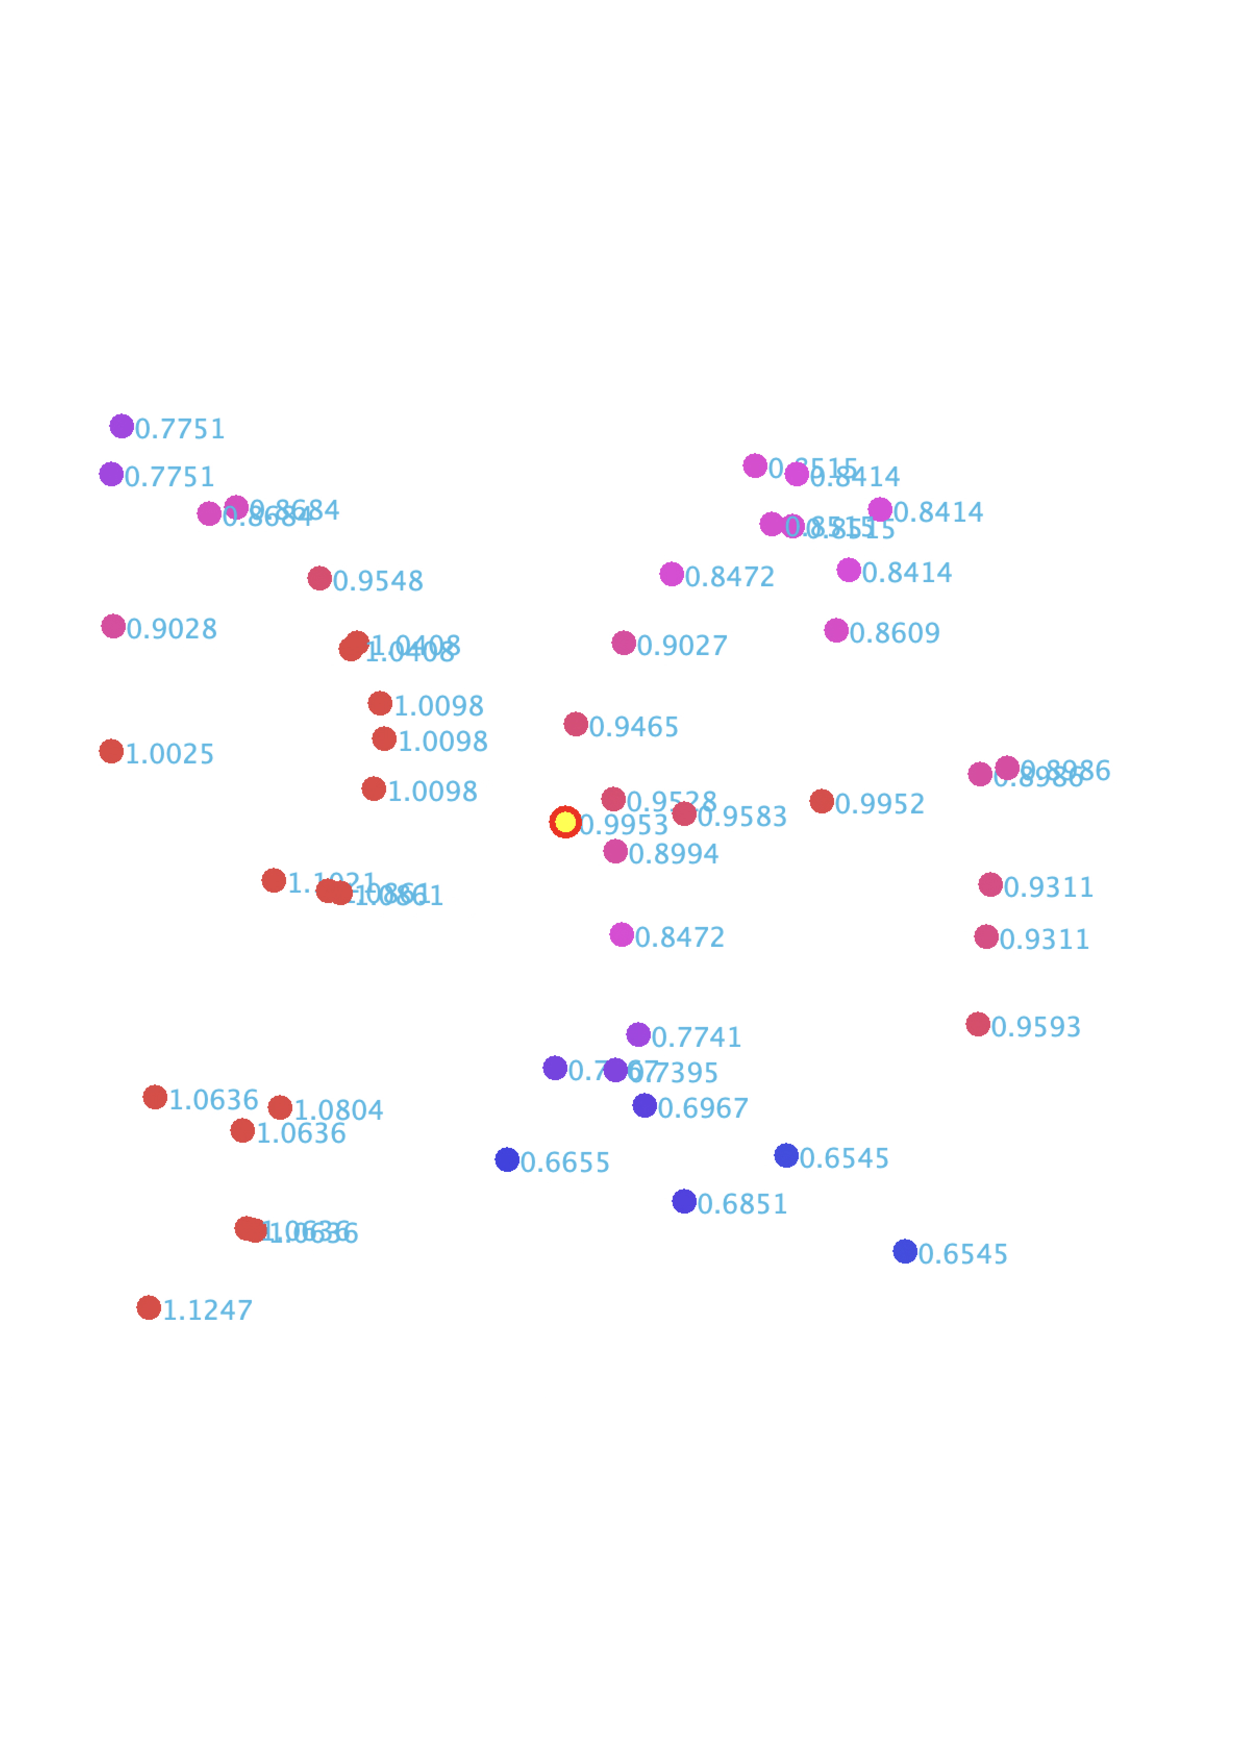
\includegraphics[width=.8\linewidth]{figures/localAverageSimulation.pdf}
    \caption{Simulazione dell'esperimento in \cref{lst:localaverageck}.
     I dispositivi inizializzano \texttt{v} casualmente e convergono verso il valore medio locale.
     Il colore dei nodi dipende dalla norma euclidea del vettore calcolato, la cui intensità è indicata a fianco.}
    \label{fig:local-average-simulation}
\end{figure}

\newpage
\section{Nel Cerchio}
\label{sec:incircle}

\paragraph{Obiettivo} Determinare se un dispositivo appartiene a una regione circolare, dati il centro e il raggio del cerchio.

% TODO (Richiede in ingresso un valore booleano che indica se il dispositivo è il centro del cerchio)
\paragraph{Codice originale} La funzione \texttt{in-circle} (\Cref{lst:incircle}) richiede in ingresso le coordinate del centro (\texttt{o}) e il raggio (\texttt{r}) del cerchio.

% TODO (Permalink)
\lstinputlisting[
    language=Lisp,
    label={lst:incircle},
    caption={Codice della funzione \texttt{in-circle} in Proto.}
]{listings/proto/in-circle.proto}
%
L'istruzione \texttt{let ((dv (- (probe (coord) 1) o)))} calcola la differenza tra le coordinate del dispositivo corrente e quelle del nodo centrale, 
depositando il risultato nella variabile \texttt{dv}.
%
Successivamente, l'espressione \texttt{(< (probe (vdot dv dv) 0) (* r r))}  verifica che il prodotto scalare di \texttt{dv} con sè stesso sia inferiore al quadrato del raggio \texttt{r}, restituendo un valore booleano   che indica l'appartenenza al cerchio.

% TODO (Aggiungere giuste reference, far vedere la funzione distanceToSquared)
\paragraph{Trasposizione in Collektive} (\Cref{lst:incircleck}) La propagazione delle coordinate del nodo centrale è realizzata tramite la funzione \texttt{gradientCast} (\Cref{lst:gradientcast}). 
In seguito, si verifica che il quadrato della distanza tra il dispositivo corrente e il centro sia inferiore al quadrato del raggio.

In \cref{fig:in-circle-simulation} è mostrata la simulazione dell'esperimento: il centro \texttt{o} è evidenziato in verde, mentre i dispositivi all'interno del cerchio sono colorati in rosso.
\lstinputlisting[
    language=Kotlin,
    label={lst:incircleck},
    caption={Trasposizione della funzione \texttt{in-circle} in Collektive.}
]{listings/collektive/inCircle.kt}

\begin{figure}
    \centering
    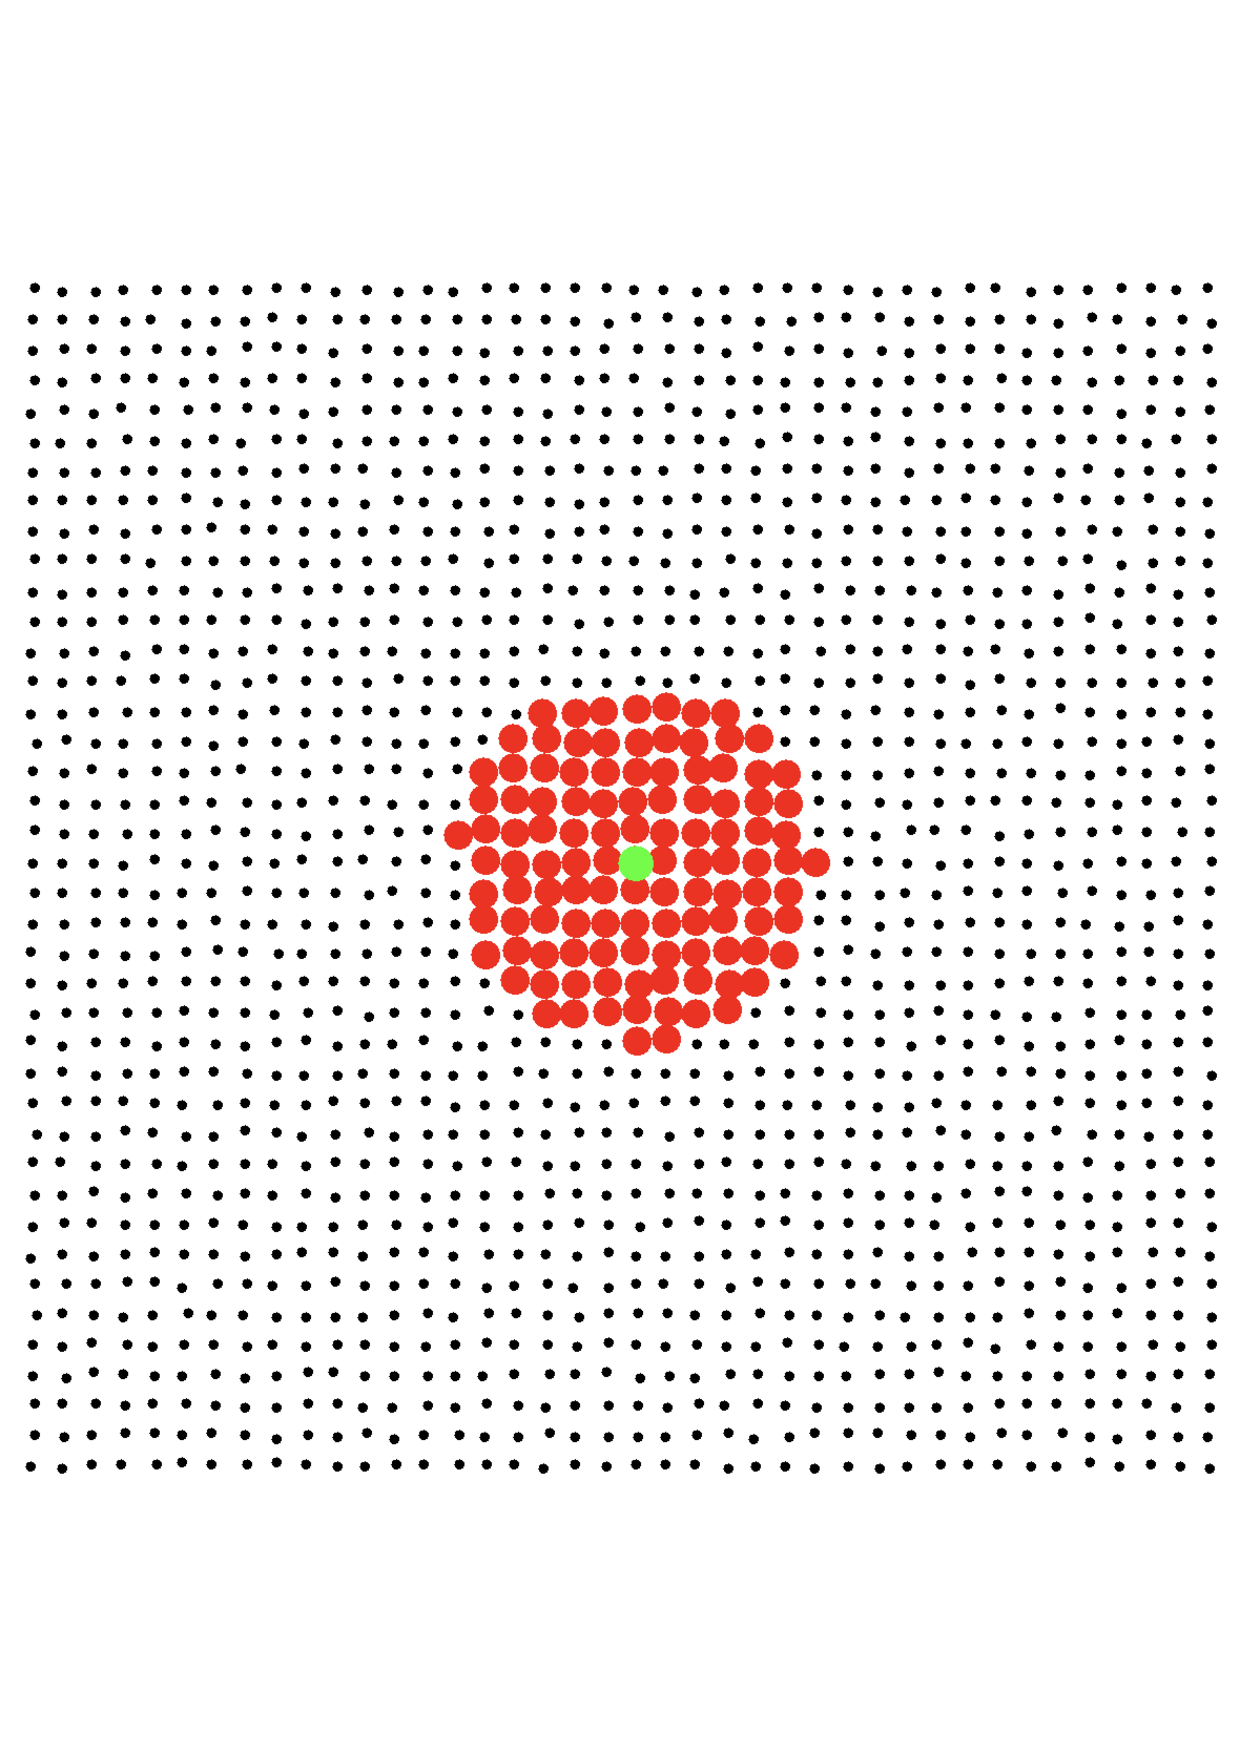
\includegraphics[width=.8\linewidth]{figures/in-circle.pdf}
    \caption{Simulazione dell'esperimento in \cref{lst:incircleck}.
    Il centro \texttt{o} è rappresentato dal dispositivo in verde, mentre i dispositivi
    all'interno del cerchio sono colorati in rosso.}
    \label{fig:in-circle-simulation}
\end{figure}

\newpage
\section{Anello}
\label{sec:ring}

\paragraph{Obiettivo} Identificare i dispositivi disposti lungo un anello di raggio variabile nel tempo.

\paragraph{Codice originale} La funzione \texttt{ring} (\Cref{lst:ring}) non prevede argomenti in ingresso, ma si avvale della funzione \texttt{sense} per individuare i dispositivi che fungono da sorgente del segnale.
%
\lstinputlisting[
    language=Lisp,
    label={lst:ring},
    caption={Codice della funzione \texttt{ring} in Proto.}
]{listings/proto/ring.proto}
%
L'espressione \texttt{(let (\dots))} si articola in due componenti principali. La prima,
\[
\texttt{((t (probe (broadcast (sense 1) (if (sense 1) (timer) 0)) 0)))}
\]
, propaga il valore del \texttt{timer} dalle sorgenti del segnale: ogni dispositivo riceve il valore dalla sorgente più vicina e lo memorizza nella variabile \texttt{t}.
%
La seconda componente, \texttt{(d (probe (gradient (sense 1)) 1))}, calcola la distanza dalla sorgente più prossima, assegnandola alla variabile \texttt{d}.
%
Infine, l'espressione \texttt{(if (< (abs (- (* 5 t) d)) 4) (green 1) (blue 1))} verifica se la distanza \texttt{d} si discosta di meno di \(4\) unità dalla posizione dell'anello, che avanza con una velocità di \(5\) unità al secondo.
%
Se la condizione è soddisfatta, il dispositivo viene colorato di verde; altrimenti, di blu.

\paragraph{Trasposizione in Collektive} (\Cref{lst:ringck}) 
La propagazione del valore del timer dalle sorgenti avviene tramite la funzione \texttt{gradientCast} (\Cref{lst:gradientcast}), mentre la funzione \texttt{distanceTo} (\Cref{lst:distanceto}) permette a ciascun dispositivo di calcolare la distanza dalla sorgente più vicina.

Come illustrato in \cref{fig:ring-simulation}, l’anello si propaga come un’onda, originata dalla sorgente. Per evitare che la simulazione si concluda subito dopo la prima propagazione, è stata introdotta una dinamica periodica che permette all’anello di formarsi e dissolversi ciclicamente nel tempo.

\lstinputlisting[
    language=Kotlin,
    label={lst:ringck},
    caption={Trasposizione della funzione \texttt{ring} in Collektive.}
]{listings/collektive/Ring.kt}

\begin{figure}
    \centering
    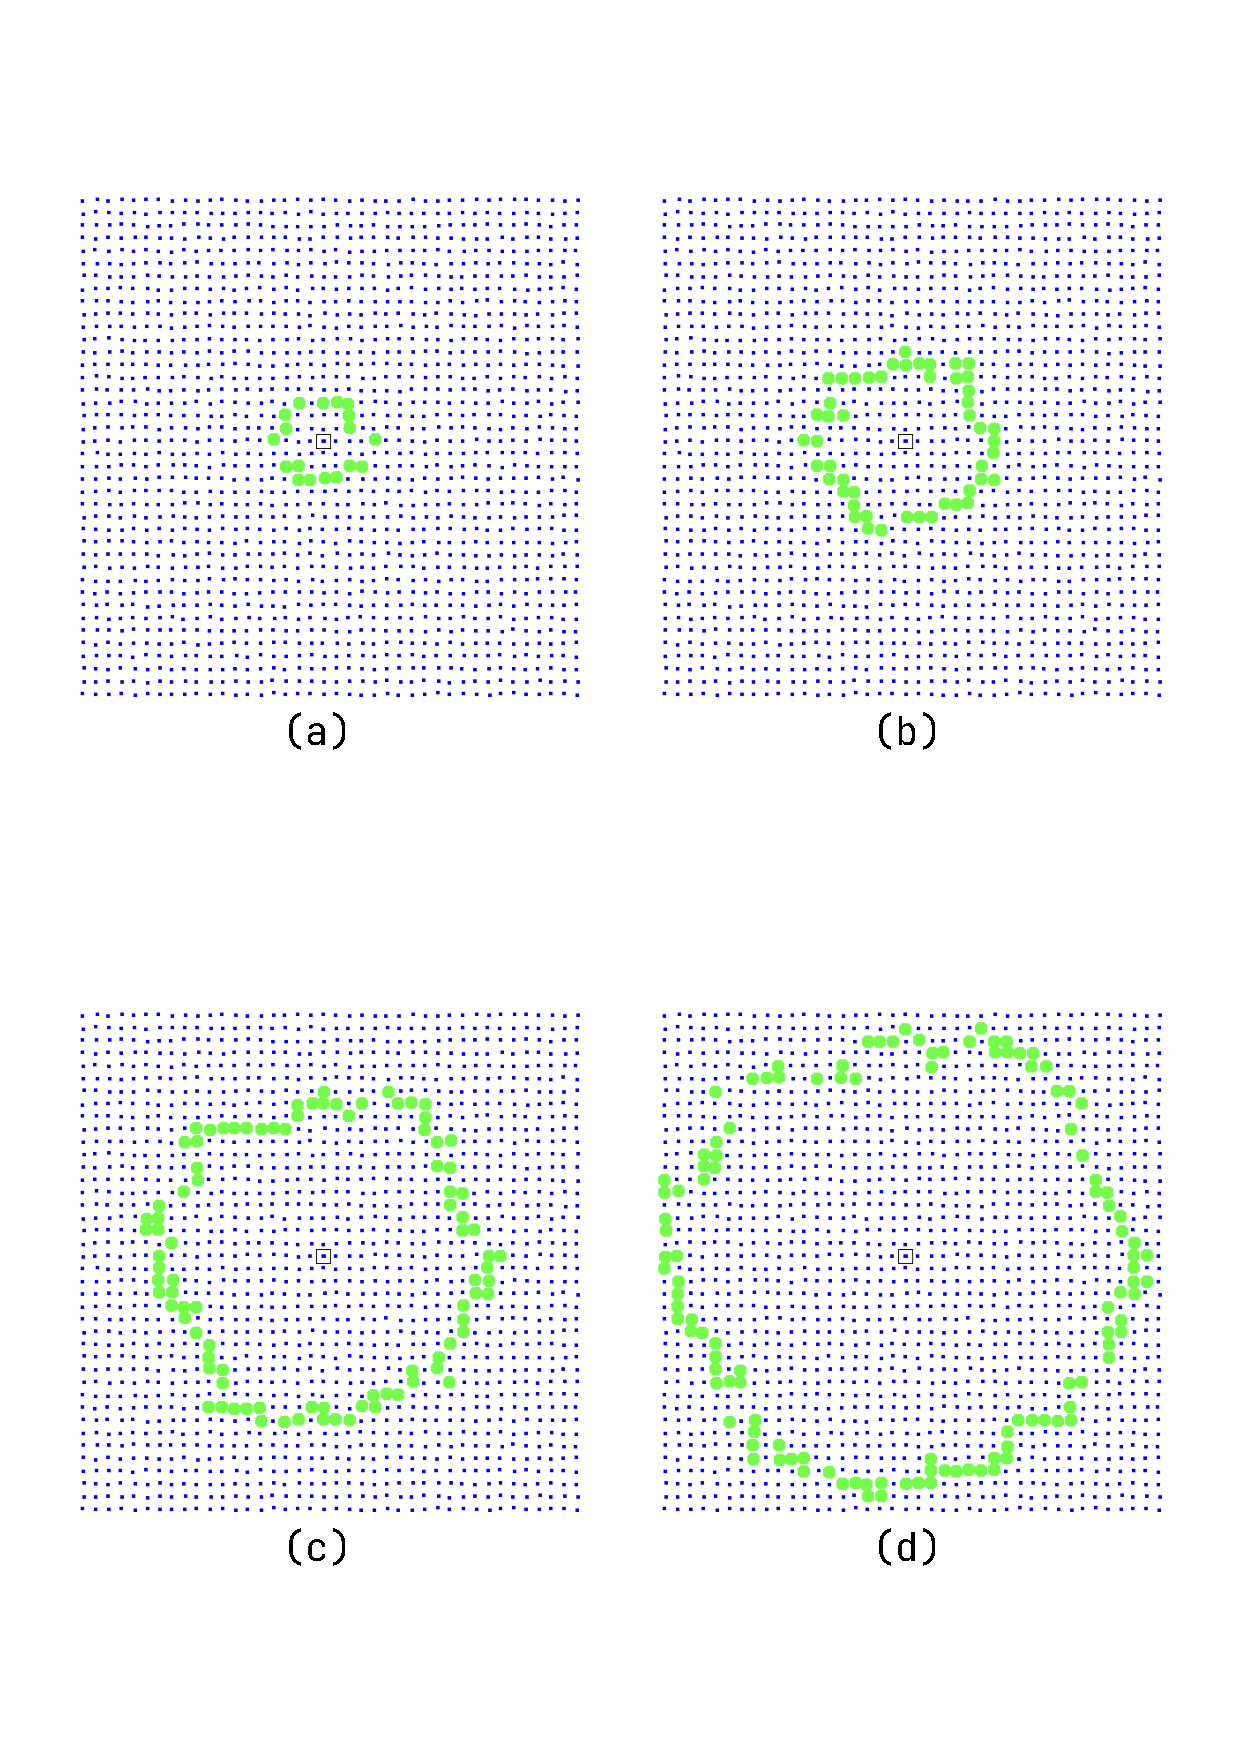
\includegraphics[width=0.8\linewidth]{figures/ring.pdf}
    \caption{Simulazione dell'esperimento in \cref{lst:ringck}.
    I dispositivi lungo l'anello sono colorati in verde, mentre gli altri sono colorati in blu.
    La simulazione è mostrata in quattro istanti temporali distinti, evidenziando il movimento dell'anello nel tempo.
    }
    \label{fig:ring-simulation}
\end{figure}

\newpage
\section{Temperature}
\label{sec:temperature}

\paragraph{Obiettivo} Simulare la diffusione del calore in un’area, considerando la presenza simultanea di sorgenti di calore e di freddo.

\paragraph{Codice originale} La funzione \texttt{temperature} (\Cref{lst:temperature}) non accetta argomenti.
Un dispositivo è una sorgente di calore se il suo identificatore \texttt{mid} è minore di \(6\) ed è pari,
mentre è una sorgente di freddo se \texttt{mid} è minore di \(6\) ma dispari.
%
\lstinputlisting[
    language=Lisp,
    label={lst:temperature},
    caption={Codice della funzione \texttt{temperature} in Proto.}
]{listings/proto/temperature.proto}
%
L'istruzione \texttt{( rep temp 25 ( mux hot 30 ( mux cold 20 (/ (sum-hood(nbr temp))(sum-hood 1)))))} modella l'evoluzione del campo di temperatura nello spazio e nel tempo.
%
Inizialmente, ogni dispositivo imposta la propria temperatura a \(25\) gradi (\texttt{rep temp 25 ...}).
%
Tale valore viene aggiornato ad ogni round in base al ruolo del dispositivo: se il nodo agisce come sorgente di calore, viene impostato a \(30\) gradi (\texttt{mux hot 30 \dots}); se invece funge da sorgente di freddo, viene fissato a \(20\) gradi (\texttt{mux cold 20 \dots}); in tutti gli altri casi, si assume la media delle temperature rilevate nel vicinato (\texttt{(/ (sum-hood(nbr temp))(sum-hood 1))}).

\paragraph{Trasposizione in Collektive} (\Cref{lst:temperatureck}) L'evoluzione spazio-temporale della temperatura è modellata tramite l'operatore \texttt{share} (\Cref{sec:collektiveshare}).

In \cref{fig:temperature-simulation} è riportata una simulazione dell'esperimento, in cui i dispositivi che agiscono come sorgenti di calore sono evidenziati da un rettangolo rosso, mentre quelli che fungono da sorgenti di freddo sono evidenziati da un rettangolo blu. Il colore di ciascun dispositivo rappresenta la temperatura locale, secondo una scala cromatica che va dal nero (freddo) al rosso (caldo).



\newpage

\lstinputlisting[
    language=Kotlin,
    label={lst:temperatureck},
    caption={Trasposizione della funzione \texttt{temperature} in Collektive.}
]{listings/collektive/Temperature.kt}

\begin{figure}
    \centering
    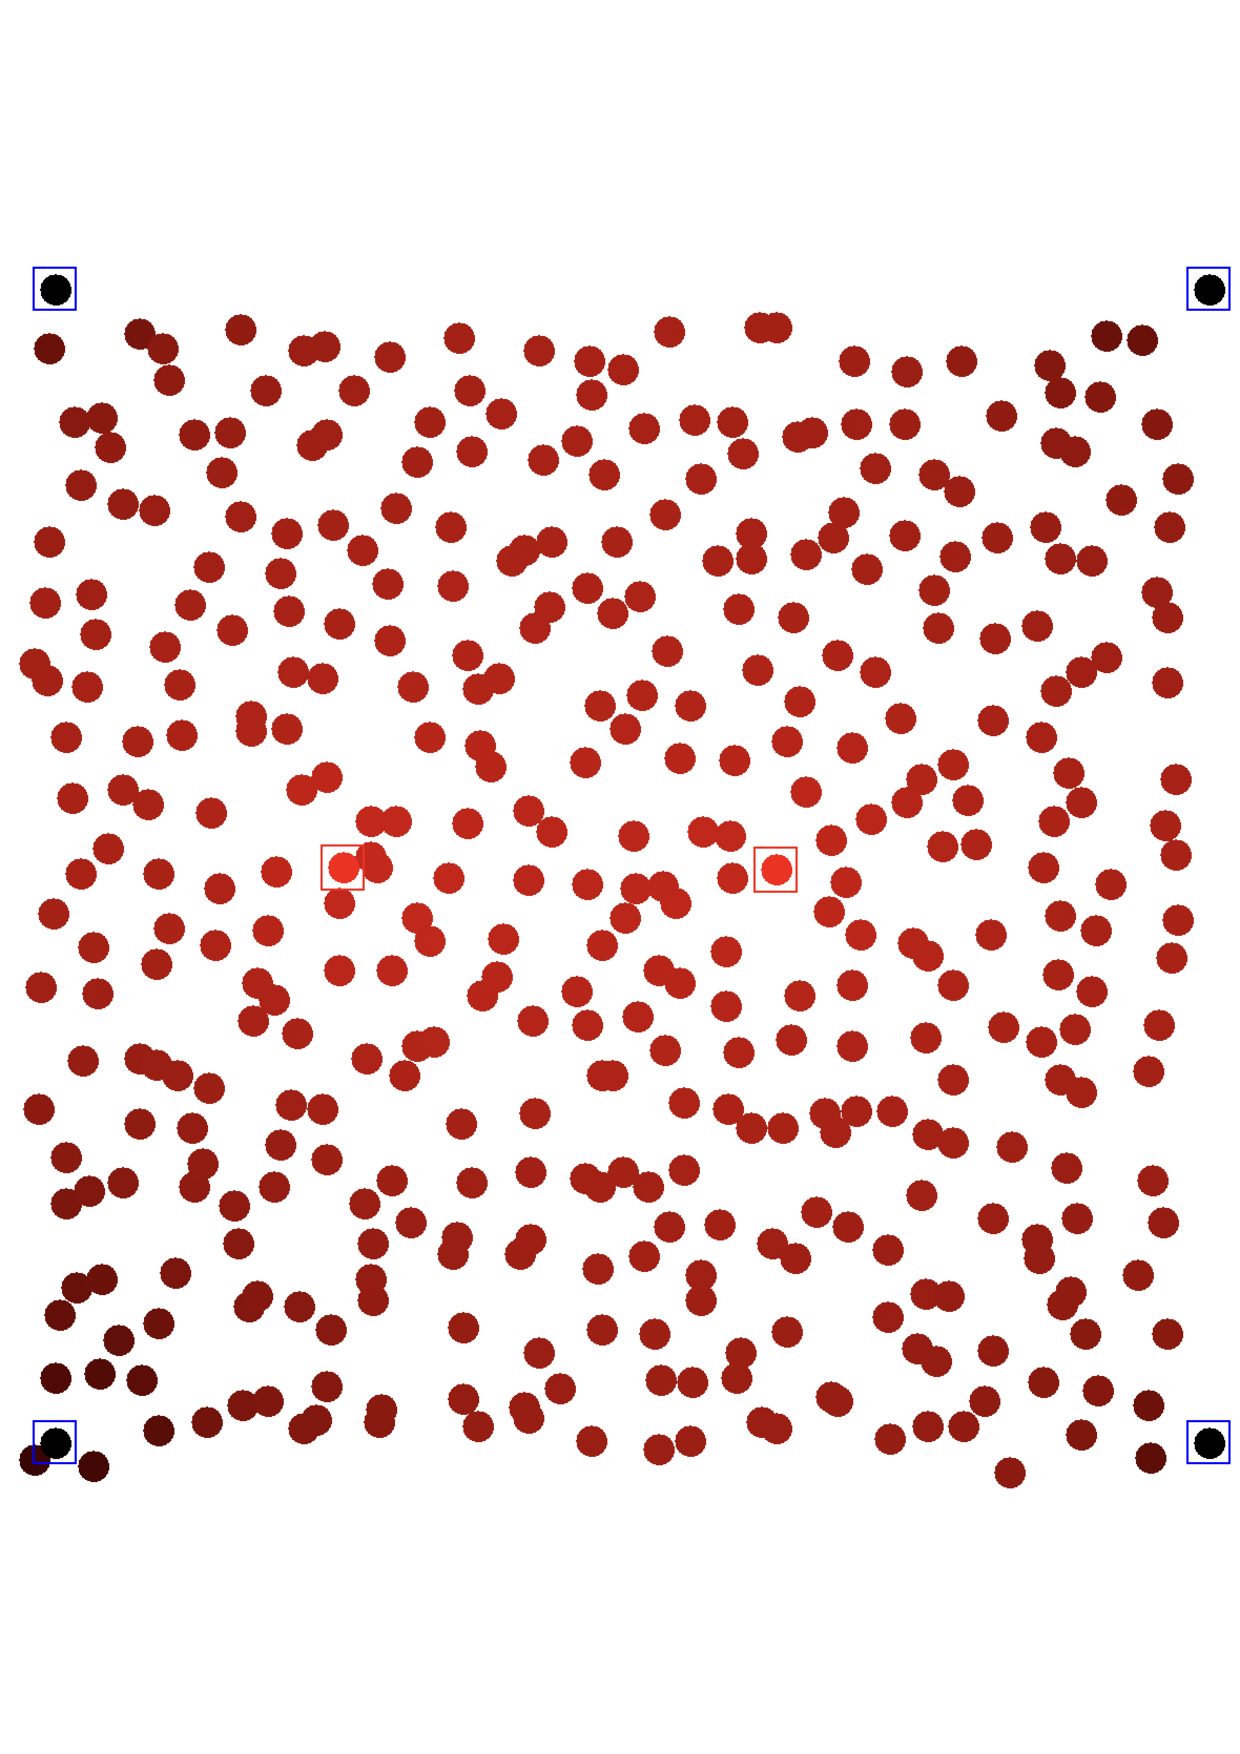
\includegraphics[width=.8\linewidth]{figures/temperature2.pdf}
    \caption{Simulazione dell'esperimento in \cref{lst:temperatureck}.
    I dispositivi che agiscono come sorgenti di calore sono evidenziati da
    un rettangolo rosso, mentre quelli che agiscono come sorgenti di freddo
    sono evidenziati da un rettangolo blu.
    Il colore dei dispositivi rappresenta la propria temperatura,
    con una scala che va dal nero (freddo) al rosso (caldo).
    }
    \label{fig:temperature-simulation}
\end{figure}

\newpage
\section{Navigazione del Gradiente}
\label{sec:navgrad}

\paragraph{Obiettivo} Guidare i nodi mobili verso una fonte di interesse all’interno della rete, muovendosi lungo la discesa del gradiente del campo delle distanze.

\paragraph{Codice originale} Il programma (\Cref{lst:navgrad}) è composto da tre funzioni: \texttt{grad}, \texttt{share-distance-to} e \texttt{nav-grad}.
%
\lstinputlisting[
    language=Lisp,
    label={lst:navgrad},
    caption={Codice Proto per l'esperimento di navigazione del gradiente, comprendente le funzioni \texttt{grad}, \texttt{share-distance-to} e \texttt{nav-grad}.}
]{listings/proto/nav-grad.proto}

\texttt{grad} calcola il gradiente di un campo di valori scalari \texttt{v}, restituendo un vettore che indica la direzione del massimo decremento di quel campo.
%
L'espressione più esterna consiste in una moltiplicazione (\texttt{*}) tra un fattore di normalizzazione e l'integrale che aggrega i contributi dei vicini al gradiente. 
%
Il fattore di normalizzazione, definito come \texttt{(/ 1 (int-hood 1))}, calcola il reciproco del numero di vicini (pesati) considerati nell'integrale.
%
Il contributo di ciascun nodo viene determinato mediante l'espressione \texttt{int-hood (if \dots)}.
%
Per ogni membro del vicinato, viene valutata la condizione \texttt{(or (= (nbr-range) 0) (not (< (abs (- v (nbr v))) (inf))))}. Se la distanza è nulla (indicando il dispositivo stesso) oppure se la differenza tra il valore locale \texttt{v} e quello del vicino è indefinita, il contributo viene azzerato per evitare singolarità.%
%
Altrimenti, si calcola mediante l’espressione \texttt{(* (/ (- v (nbr v)) (nbr-range)) (normalize (nbr-vec))))}, che corrisponde al prodotto tra la differenza dei valori del campo, normalizzata rispetto alla distanza tra i due dispositivi, e il vettore normalizzato direzionato verso il vicino.

\texttt{share-distance-to} calcola e condivide una stima della distanza dalla sorgente all’interno della rete. Essa richiede due argomenti booleani: \texttt{is-calculating}, che indica se il dispositivo è abilitato al calcolo della distanza, e \texttt{source}, che identifica i dispositivi di cui si vuole conoscere la distanza.
%
I nodi abilitati al calcolo sfruttano la funzione \texttt{distance-to} per stimare la distanza dalla sorgente, memorizzando il risultato nella variabile \texttt{base}.
%
I dispositivi per cui \texttt{base} risulta finito vengono illuminati di verde.
%
La funzione restituisce il risultato dell'espressione \texttt{(mux is-calculating base (min-hood (+ (nbr-range) (nbr base))))}.
\\
Se \texttt{is-calculating} è vero, la funzione restituisce \texttt{base}; altrimenti, restituisce il minimo tra le somme delle distanze dai vicini e le rispettive stime di distanza dalla sorgente.

La funzione \texttt{nav-grad} combina le funzionalità di \texttt{share-distance-to} e \texttt{grad} per calcolare il vettore di navigazione verso la sorgente.
%
Richiede in ingresso \texttt{is-mover}, il quale indica la mobilità del dispositivo, e \texttt{source}, che identifica i dispositivi sorgente del campo di distanza.
%
Il gradiente del campo viene calcolato tramite l’espressione \texttt{(grad (share-distance-to (not is-mover) source))} e il risultato viene memorizzato nella variabile \texttt{g}.
%
Si restituisce il risultato di \texttt{(mux (and is-mover (> (len g) 0)) (normalize g) (tup 0 0)}.
%
Se il dispositivo è mobile e \texttt{g} ha lunghezza positiva, l'esito è il vettore normalizzato \texttt{g}; altrimenti, si ottiene il vettore nullo.
\paragraph{Trasposizione in Collektive} La funzione \texttt{grad} (\Cref{lst:gradck}) è stata tradotta come segue : si calcolano le differenze (\texttt{differences}) tra il valore locale e quelli dei vicini tramite l'espressione \texttt{mapNeighborhood \{ v \} - neighboring(v)} (\Cref{lst:collektivenbrexamples}), quindi si determinano distanze e direzioni rispetto ai vicini e si combinano questi campi di vicinato (\texttt{alignedMapValues}) per ottenere il gradiente.

La funzione \texttt{shareDistanceTo} (\Cref{lst:sharedistancetock}) utilizza la funzione \texttt{distanceTo} (\Cref{lst:distanceto}) per calcolare le distanze dalla sorgente; i dispositivi incapaci di calcolarla determinano il minimo tra la somma delle distanze dai vicini e le rispettive stime (\texttt{neighborDistances() + neighboring(myDist)}) , grazie all'espressione \texttt{potentialDist.all.valueOfMinBy(\dots)}.

In \Cref{lst:navgradck} si mostra la trasposizione della funzione \texttt{nav-grad} che, come l'originale, combina le funzionalità delle due funzioni precedenti per calcolare il vettore di navigazione verso la sorgente.

\lstinputlisting[
    language=Kotlin,
    label={lst:gradck},
    caption={Trasposizione della funzione \texttt{grad} in Collektive.}
]{listings/collektive/Grad.kt}

\lstinputlisting[
    language=Kotlin,
    label={lst:sharedistancetock},
    caption={Trasposizione della funzione \texttt{share-distance-to} in Collektive.}
]{listings/collektive/ShareDistanceTo.kt}

\newpage
\lstinputlisting[
    language=Kotlin,
    label={lst:navgradck},
    caption={Trasposizione della funzione \texttt{nav-grad} (\ref{lst:navgrad}) in Collektive.}
]{listings/collektive/NavGrad.kt}

In \cref{fig:navgrad-simulation} è riportata la simulazione dell'esperimento, in cui ogni nodo è colorato in base alla distanza dalla sorgente (evidenziata in rosso), mentre i dispositivi mobili sono evidenziati in blu. La figura mostra come i nodi mobili seguano la discesa del gradiente del campo delle distanze per raggiungere la sorgente. 

\begin{figure}
    \centering
    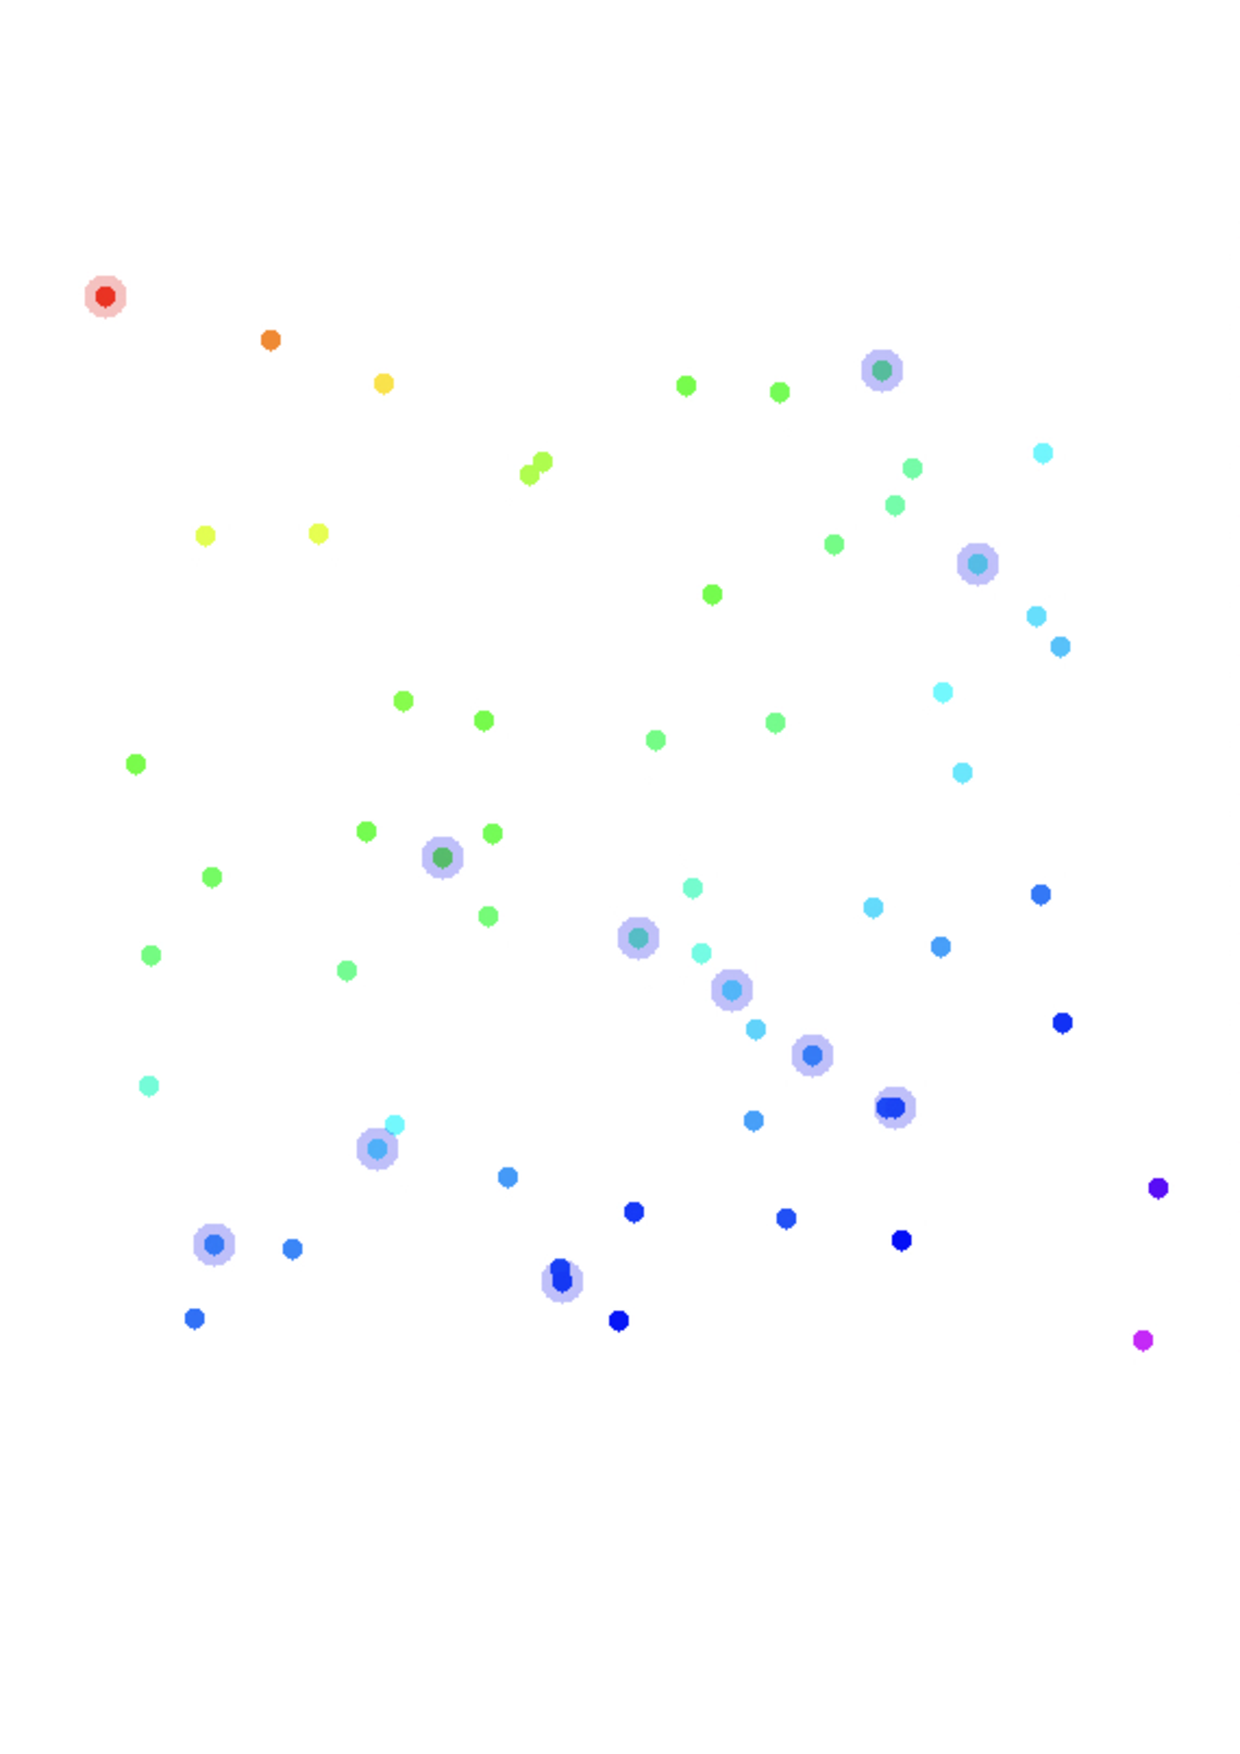
\includegraphics[width=.8\linewidth]{figures/navgrad.pdf}
    \caption{Simulazione dell'esperimento in \cref{lst:navgradck}.
    Ogni nodo è colorato rispetto alla distanza dalla sorgente (nodo evidenziato in rosso).
    I dispositivi mobili sono evidenziati da un cerchio blu.
    }
    \label{fig:navgrad-simulation}
\end{figure}

\newpage
\section{Partizionamento di Voronoi}
\label{sec:voronoi}

\paragraph{Obiettivo} Suddividere lo spazio della rete tramite partizionamento di Voronoi.
%
Un insieme di dispositivi è designato come sorgenti.
%
Ogni altro nodo determina a quale sorgente è più vicino, suddividendo di fatto lo spazio della rete in celle. 
%
Il dispositivo è classificato in base alla sua posizione: in una cella, su un bordo (tra due celle) o come vertice (all'intersezione di almeno tre celle).
%
La colorazione dei nodi riflette questa classificazione.

\paragraph{Codice originale} Il programma (\Cref{lst:voronoi}) richiede in ingresso due valori booleani: \texttt{src}, che definisce l'insieme dei dispositivi generatori delle celle, e \texttt{showedge}, un flag che abilita la visualizzazione dei bordi.
%
\lstinputlisting[
    language=Lisp,
    label={lst:voronoi},
    caption={Codice della funzione \texttt{voronoi} in Proto.}
]{listings/proto/voronoi.proto}
%
Tramite il costrutto \texttt{let*}, si definiscono tre variabili in modo sequenziale:
\begin{itemize}
    \item \texttt{closest-src}: identificatore del dispositivo sorgente più vicino, sfruttando la funzione \texttt{broardcast src (mid)}.
    \item \texttt{edge}: indica se il dispositivo corrente si trovi su un bordo tra due celle, ossia se esista almeno un vicino (\texttt{any-hood}) la cui sorgente più prossima (\texttt{nbr closest-src}) sia diversa dalla propria (\texttt{closest-src}).
    \item \texttt{vertex}: indica se il dispositivo corrente sia un vertice, ossia se si trovi su un bordo (\texttt{and edge}) e, tra i vicini appartenenti a celle diverse (\texttt{max-nbr}, \texttt{min-nbr}), vi siano almeno due identificativi di sorgente distinti (\texttt{(not (= max-nbr min-nbr))}).
\end{itemize}
%
Se il flag \texttt{showedge} è attivo, i dispositivi vengono colorati in base alla loro classificazione: i vertici assumono il colore \texttt{rgb (tup 1 0 0)}, i bordi \texttt{rgb (tup 0 0 0.5)}, mentre gli altri dispositivi adottano il colore associato alla propria cella di appartenenza (\texttt{uid2rgb closest-src 10}).
%
La funzione restituisce la coppia \texttt{(tup closest-src edge)}.

\paragraph{Trasposizione in Collektive} (\Cref{lst:voronoick}) L'identificatore della sorgente più vicina è determinato dalla funzione \texttt{gradientCast} (\Cref{lst:gradientcast}), la cui natura assicura che ogni dispositivo ottenga il valore da quella più prossima.

I vicini condividono il valore calcolato tramite \texttt{neighboring} (\Cref{lst:collektivenbr}), permettendo a ogni nodo di contare il numero di sorgenti diverse nel vicinato, determinando così la propria classificazione.
%
Se \texttt{distinctSources >= 3}, il dispositivo è un vertice; se \texttt{distinctSources == 2}, è su un bordo.

In questa traduzione, il programma non restituisce la coppia \texttt{(closest-src edge)}, bensì si limita a restituire il colore (\Cref{fig:voronoi-simulation}) associato al dispositivo.

\newpage
\lstinputlisting[
    language=Kotlin,
    label={lst:voronoick},
    caption={Trasposizione della funzione \texttt{voronoi} in Collektive.}
]{listings/collektive/Voronoi.kt}

\begin{figure}
    \centering
    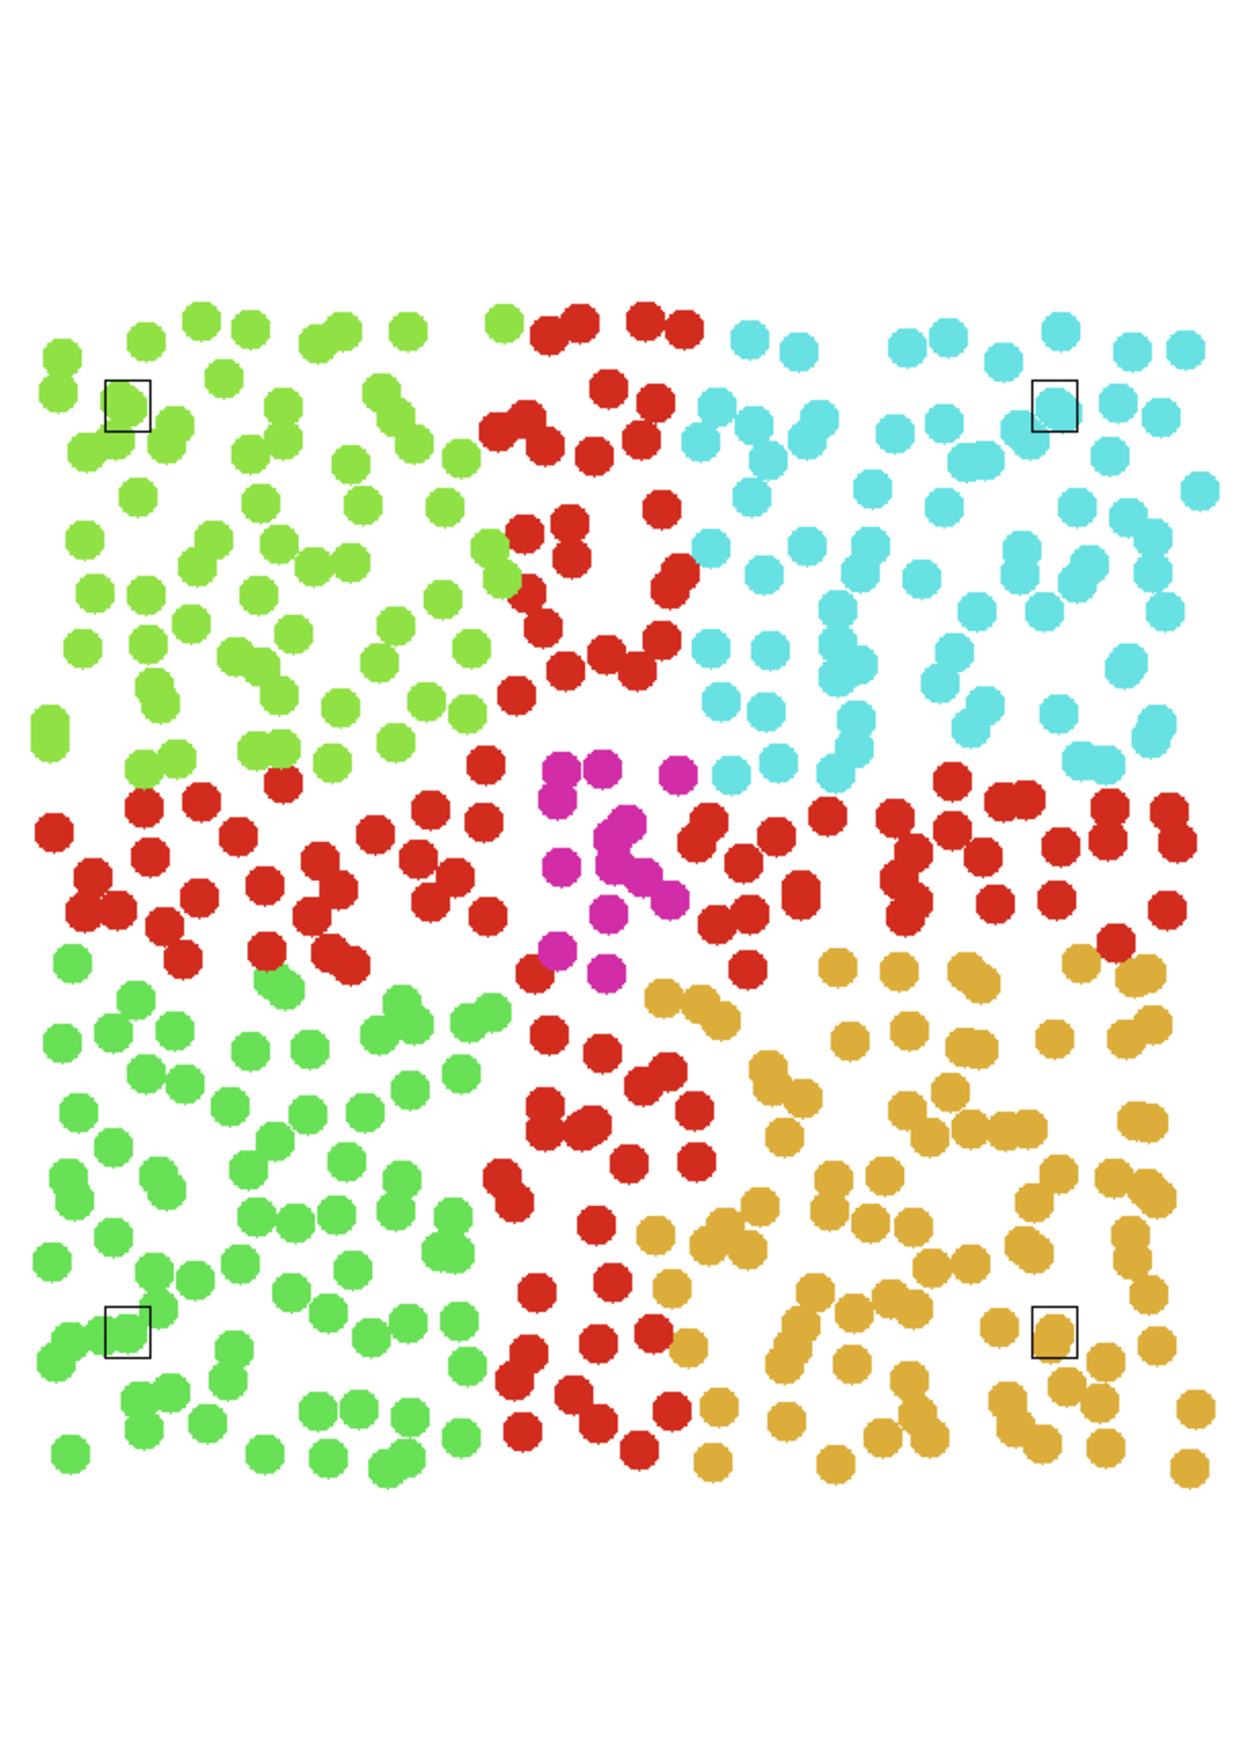
\includegraphics[width=.8\linewidth]{figures/voronoi.pdf}
    \caption{Simulazione dell'esperimento in \cref{lst:voronoick}.
    I dispositivi sono colorati in base alla cella di appartenenza:
    i dispositivi sui bordi sono colorati in rosso,
    mentre i vertici sono colorati in magenta.
    Le sorgenti sono evidenziate da un rettangolo nero.
    }
    \label{fig:voronoi-simulation}
\end{figure}

\newpage
\section{Connessione lungo l'albero dei cammini minimi}
\label{sec:wire}

\paragraph{Obiettivo} Stabilire un collegamento tra due dispositivi, identificando e attraversando i nodi che compongono l'albero dei cammini minimi che li collega.

\paragraph{Codice originale} Il programma è costituito da tre funzioni: \texttt{spath}, \texttt{connect} e \texttt{wire}.

La funzione \texttt{spath} (\Cref{lst:spath}) determina l'albero dei cammini minimi tra sorgente (\texttt{src}) e destinazione (\texttt{dest}), sfruttando la distanza \texttt{d} di ciascun dispositivo rispetto alla destinazione.

In fase iniziale, viene definita la variabile \texttt{min-id}, la quale memorizza l'identificatore del vicino che presenta la distanza minima \texttt{d}, come espresso da \texttt{(2nd (min-hood (tup (nbr d) (nbr (mid)))))}.

Successivamente, l'espressione \texttt{(rep ispath \dots)} tiene traccia dei dispositivi che appartengono all'albero. La variabile \texttt{ispath} è inizializzata a \texttt{0} (\texttt{false}) e viene aggiornata a ogni round mediante l'espressione:
\[
\texttt{(mux src 1 (any-hood (muxand (= (mid) (nbr min-id) (nbr ispath)))))}
\]
Questa logica opera come segue:
\begin{itemize}
    \item Se il dispositivo corrente è la sorgente (\texttt{src}), \texttt{ispath} è impostato a \texttt{1} (\texttt{true}).
    \item Altrimenti, il dispositivo verifica se almeno un vicino (\texttt{any-hood}) soddisfa congiuntamente due condizioni: che il proprio identificatore (\texttt{(mid)}) sia il \texttt{min-id} del vicino (\texttt{= (mid) (nbr min-id)}), e che tale vicino faccia già parte dell'albero (\texttt{(nbr ispath)}).
\end{itemize}

La funzione restituisce \texttt{ispath}.
%
\newpage
\lstinputlisting[
    language=Lisp,
    label={lst:spath},
    caption={Codice della funzione \texttt{spath} in Proto.}
]{listings/proto/spath.proto}

\texttt{connect} (\Cref{lst:connect}) stabilisce il collegamento logico tra sorgente (\texttt{src}) e destinazione (\texttt{dest}), computando un vettore di connessione che indica il prossimo dispositivo lungo l'albero.

Ogni dispositivo calcola innanzitutto la propria distanza \texttt{d} dalla destinazione mediante la funzione \texttt{distance-to}. Successivamente, tutti i dispositivi verificano la propria appartenenza all'albero, invocando \texttt{spath}.

Attraverso l'espressione \texttt{if thepath \dots}, i dispositivi che risultano parte dell'albero collaborano per calcolare il vettore di connessione. Questo calcolo è basato sulla ricerca della distanza minima rispetto alla destinazione tra i nodi vicini (\texttt{(min-hood (nbr d))}). Vengono poi sommati i contributi di quei vicini per cui la distanza \texttt{(nbr d)} coincida con tale distanza (\texttt{= (nbr d) min-d}).

Se tale condizione è verificata, l'espressione \texttt{mux \dots} restituisce il vettore che punta verso il vicino in questione (\texttt{(nbr-vec)}); in caso contrario, restituisce il vettore nullo.

\lstinputlisting[
    language=Lisp,
    label={lst:connect},
    caption={Codice della funzione \texttt{connect} in Proto.}
]{listings/proto/connect.proto}

La funzione \texttt{wire} (\cref{lst:wire}) invoca \texttt{connect} solo per i nodi che non hanno un ostacolo vicino (\texttt{near-obst}) oppure che siano la sorgente o la destinazione (\texttt{(and (not src) (not dest))}).

\lstinputlisting[
    language=Lisp,
    label={lst:wire},
    caption={Codice della funzione \texttt{wire} in Proto.}
]{listings/proto/wire.proto}


\paragraph{Trasposizione in Collektive} In \Cref{lst:spathck} è mostrata la trasposizione della funzione \texttt{spath}. 
%
Si utilizza il costrutto \texttt{share} (\Cref{lst:collektiveshare}) per mantenere lo stato di appartenenza all'albero, condividendolo allo stesso tempo con i nodi adiacenti e ottenendo così una vista sul loro stato (\texttt{nbrIsPath}).
%
L'identificatore del vicino con distanza minima dalla destinazione si ottiene costruendo un \texttt{Field} che associa a ciascun nodo del vicinato la sua distanza (\texttt{neighboring(toDestination)} (\Cref{lst:collektivenbr})), e selezionando l'identificatore corrispondente al valore minimo tramite \texttt{.minBy \{ (\_, value) -> value \}.id}.
%
Successivamente, si costruisce un \texttt{Field} di \texttt{minId}, che viene trasformato in un campo di valori booleani: il valore è \texttt{true} per i nodi il cui \texttt{minId} coincide con il proprio identificatore. Questo campo viene quindi combinato con \texttt{nbrIsPath} tramite un'operazione logica \texttt{and}; se almeno un nodo adiacente restituisce \texttt{true}, il dispositivo viene considerato parte dell'albero.

La corrispondente implementazione di \texttt{connect} è riportata in \Cref{lst:connectck}.
%
Ogni nodo calcola la distanza dalla destinazione tramite \texttt{distanceTo} (\Cref{lst:distanceto}) e verifica la propria appartenenza all'albero di percorso minimo invocando la funzione \texttt{shortestPath}.
%
Per calcolare il vettore di connessione, si combinano le distanze dei nodi adiacenti dalla destinazione (\texttt{neighborDistances}) con i rispettivi vettori direzionali (\texttt{neighborVectors}), considerando esclusivamente il contributo del nodo la cui distanza corrisponde al valore minimo rilevato nel vicinato.

La trasposizione della funzione \texttt{wire} è mostrata in \Cref{lst:wireck}. 
%
La presenza di ostacoli nei dintorni viene rilevata costruendo un \texttt{Field} booleano tramite \texttt{neighboring(obstacle)} (\Cref{lst:collektivenbr}) e verificando, con la funzione \texttt{any(\dots)}, se almeno uno dei nodi adiacenti rappresenta un ostacolo.

In \cref{fig:wire-simulation} è mostrata la simulazione dell'esperimento.

\newpage

\lstinputlisting[
    language=Kotlin,
    label={lst:spathck},
    caption={Trasposizione della funzione \texttt{spath} (\ref{lst:spath}) in Collektive.}
]{listings/collektive/ShortestPath.kt}

\lstinputlisting[
    language=Kotlin,
    label={lst:connectck},
    caption={Trasposizione della funzione \texttt{connect} (\ref{lst:connect}) in Collektive.}
]{listings/collektive/Connect.kt}

\lstinputlisting[
    language=Kotlin,
    label={lst:wireck},
    caption={Trasposizione della funzione \texttt{wire} (\ref{lst:wire}) in Collektive.}
]{listings/collektive/Wire.kt}


\begin{figure}
    \centering
    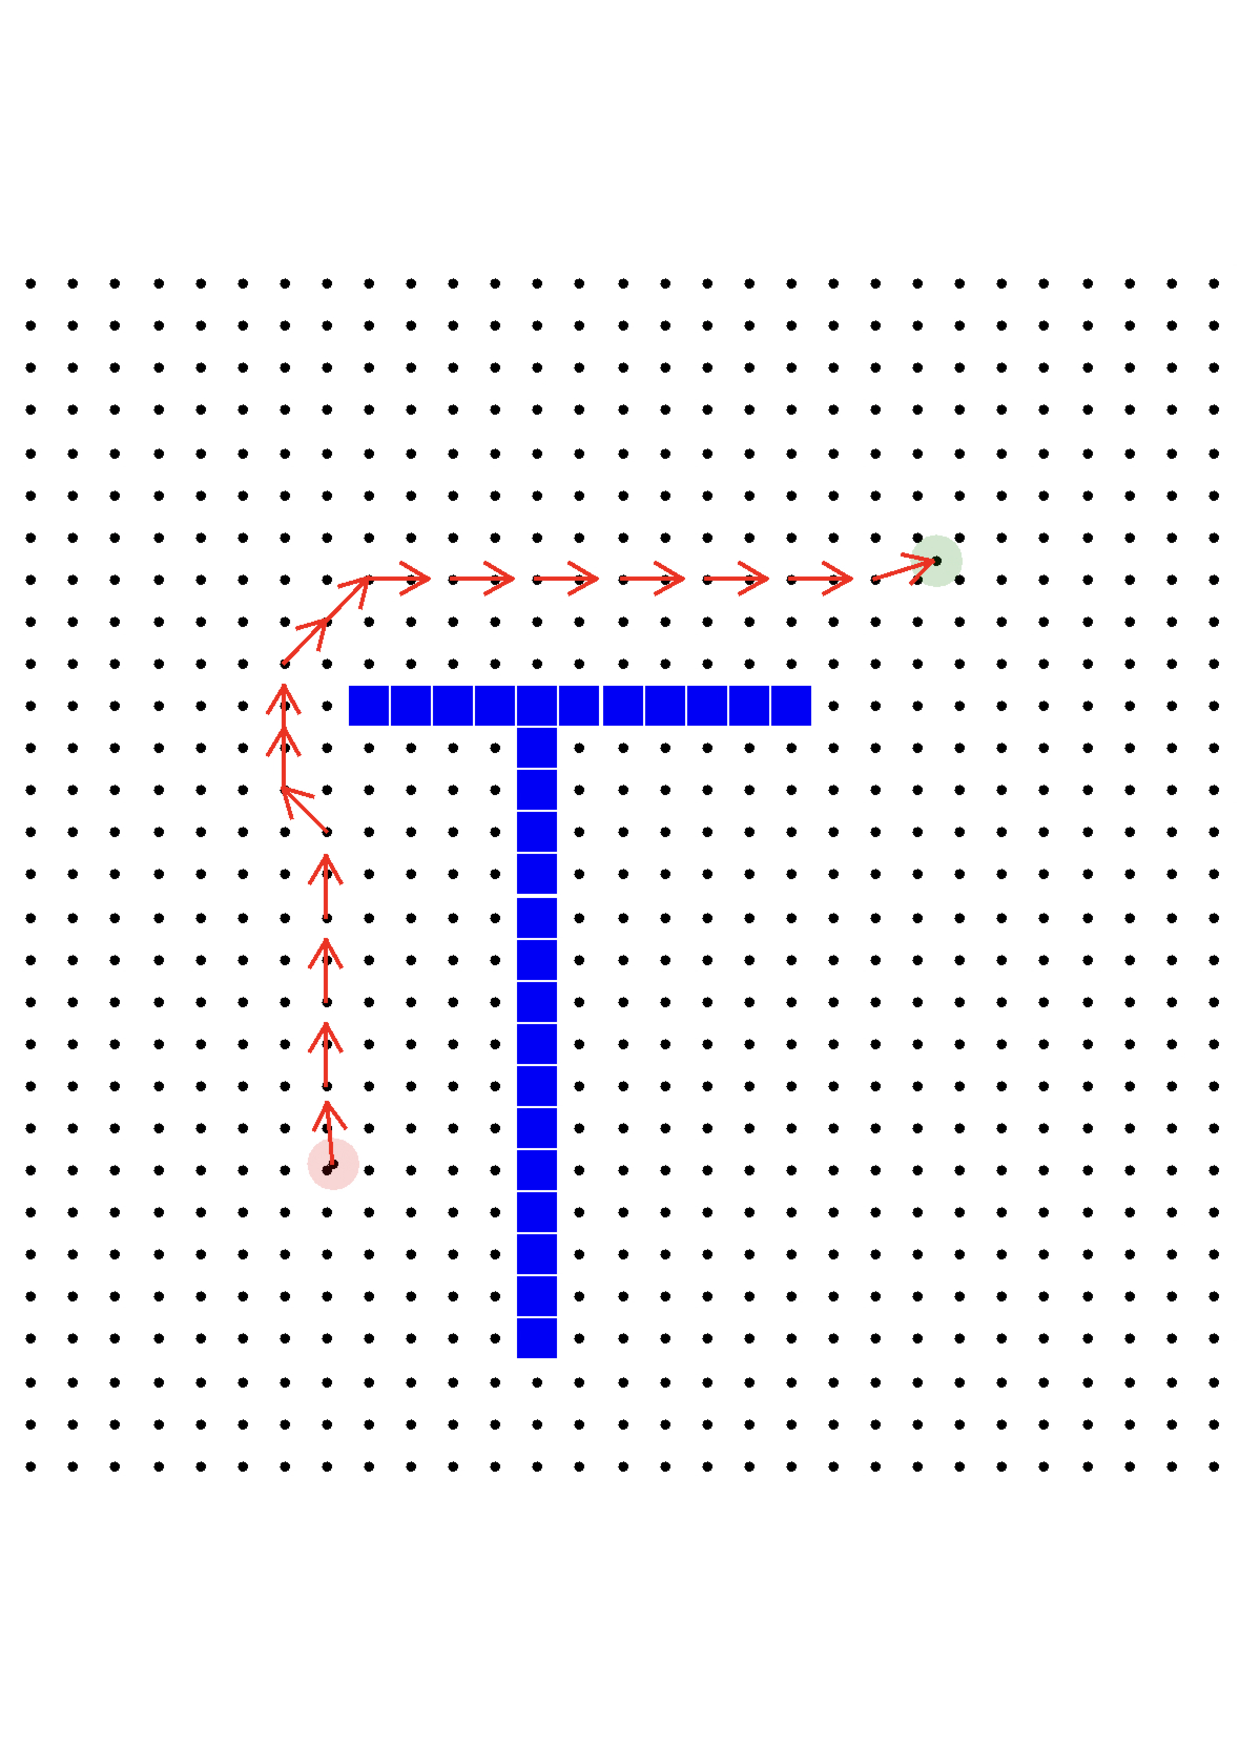
\includegraphics[width=.8\linewidth]{figures/wire2.pdf}
    \caption{Simulazione dell'esperimento in \cref{lst:wireck}.
    La sorgente è evidenziata in rosso mentre la destinazione in verde.
    Gli ostacoli sono rappresentati attraverso quadrati blu.
    I dispositivi che appartengono all'albero puntano verso il prossimo nodo del cammino, formando un collegamento che unisce sorgente e destinazione.
    }
    \label{fig:wire-simulation}
\end{figure}

\newpage
\section{Tracciamento}
\label{sec:track}

\paragraph{Obiettivo} Progettare un sistema di tracciamento in cui un dispositivo (destinazione) ne segua un altro (target), sfruttando un canale di comunicazione dedicato.

\paragraph{Codice originale} Il programma (\Cref{lst:track}) si compone di due funzioni: 
\\
\texttt{channel} e \texttt{track}.

La funzione \texttt{channel} ha lo scopo di creare un "canale" di dispositivi che collega la sorgente (\texttt{src}) alla destinazione (\texttt{dest}), restituendo \texttt{true} per tutti i nodi che fanno parte di questo percorso e \texttt{false} per gli altri. 
%
In particolare, la funzione calcola la distanza tra sorgente e destinazione (\texttt{(distance src dst)}) e considera appartenenti al canale tutti i dispositivi per cui la somma delle distanze dalla sorgente e dalla destinazione risulta minore o uguale alla distanza tra le due, incrementata di un margine di tolleranza (\texttt{(<= (+ (gradient src) (gradient dst)) (+ d 1))}).
%
Infine, la funzione restituisce \texttt{true} solo per i dispositivi effettivamente raggiungibili sia dalla sorgente sia dalla destinazione e che rientrino nella larghezza specificata dal canale, ampliata tramite la funzione \texttt{dilate}.

La funzione \texttt{track} consente alla destinazione di seguire il target sfruttando il canale creato da \texttt{channel}: la posizione del target viene propagata lungo il canale e, una volta ricevuta, la destinazione ne calcola la differenza rispetto alle proprie coordinate, determinando così la direzione verso cui puntare (\texttt{(- (broadcast target coord) coord)}).
\lstinputlisting[
    language=Lisp,
    label={lst:track},
    caption={Codice Proto per l’esperimento di navigazione del gradiente,
comprendente le funzioni \texttt{channel} e \texttt{track}.}
]{listings/proto/track.proto}

\paragraph{Trasposizione in Collektive} Per l'implementazione di \texttt{channel} è stata adottata la versione già utilizzata nella simulazione ChannelWithObstacle\footnote{\url{https://github.com/Collektive/collektive-examples/blob/fc511935fa0cce9116cd6bb8e00088443c2cd506/simulation/src/main/kotlin/it/unibo/collektive/examples/channel/ChannelWithObstacles.kt\#L28C1-L44}} (\Cref{lst:channelck}).

La propagazione delle coordinate del nodo target nella funzione \texttt{track} (\Cref{lst:trackck}) avviene tramite la funzione \texttt{gradientCast} (\Cref{lst:gradientcast}), che diffonde le informazioni esclusivamente tra i nodi appartenenti al canale, grazie al partizionamento derivato dal costrutto \texttt{when}.

\newpage
\lstinputlisting[
    language=Kotlin,
    label={lst:trackck},
    caption={Trasposizione della funzione \texttt{track} (\ref{lst:track}) in Collektive.}
]{listings/collektive/Track.kt}

\lstinputlisting[
    language=Kotlin,
    label={lst:channelck},
    caption={Funzione \texttt{channel} tratta dall'esperimento ChannelWithObstacles.}
]{listings/collektive/Channel.kt}

\begin{figure}
    \centering
    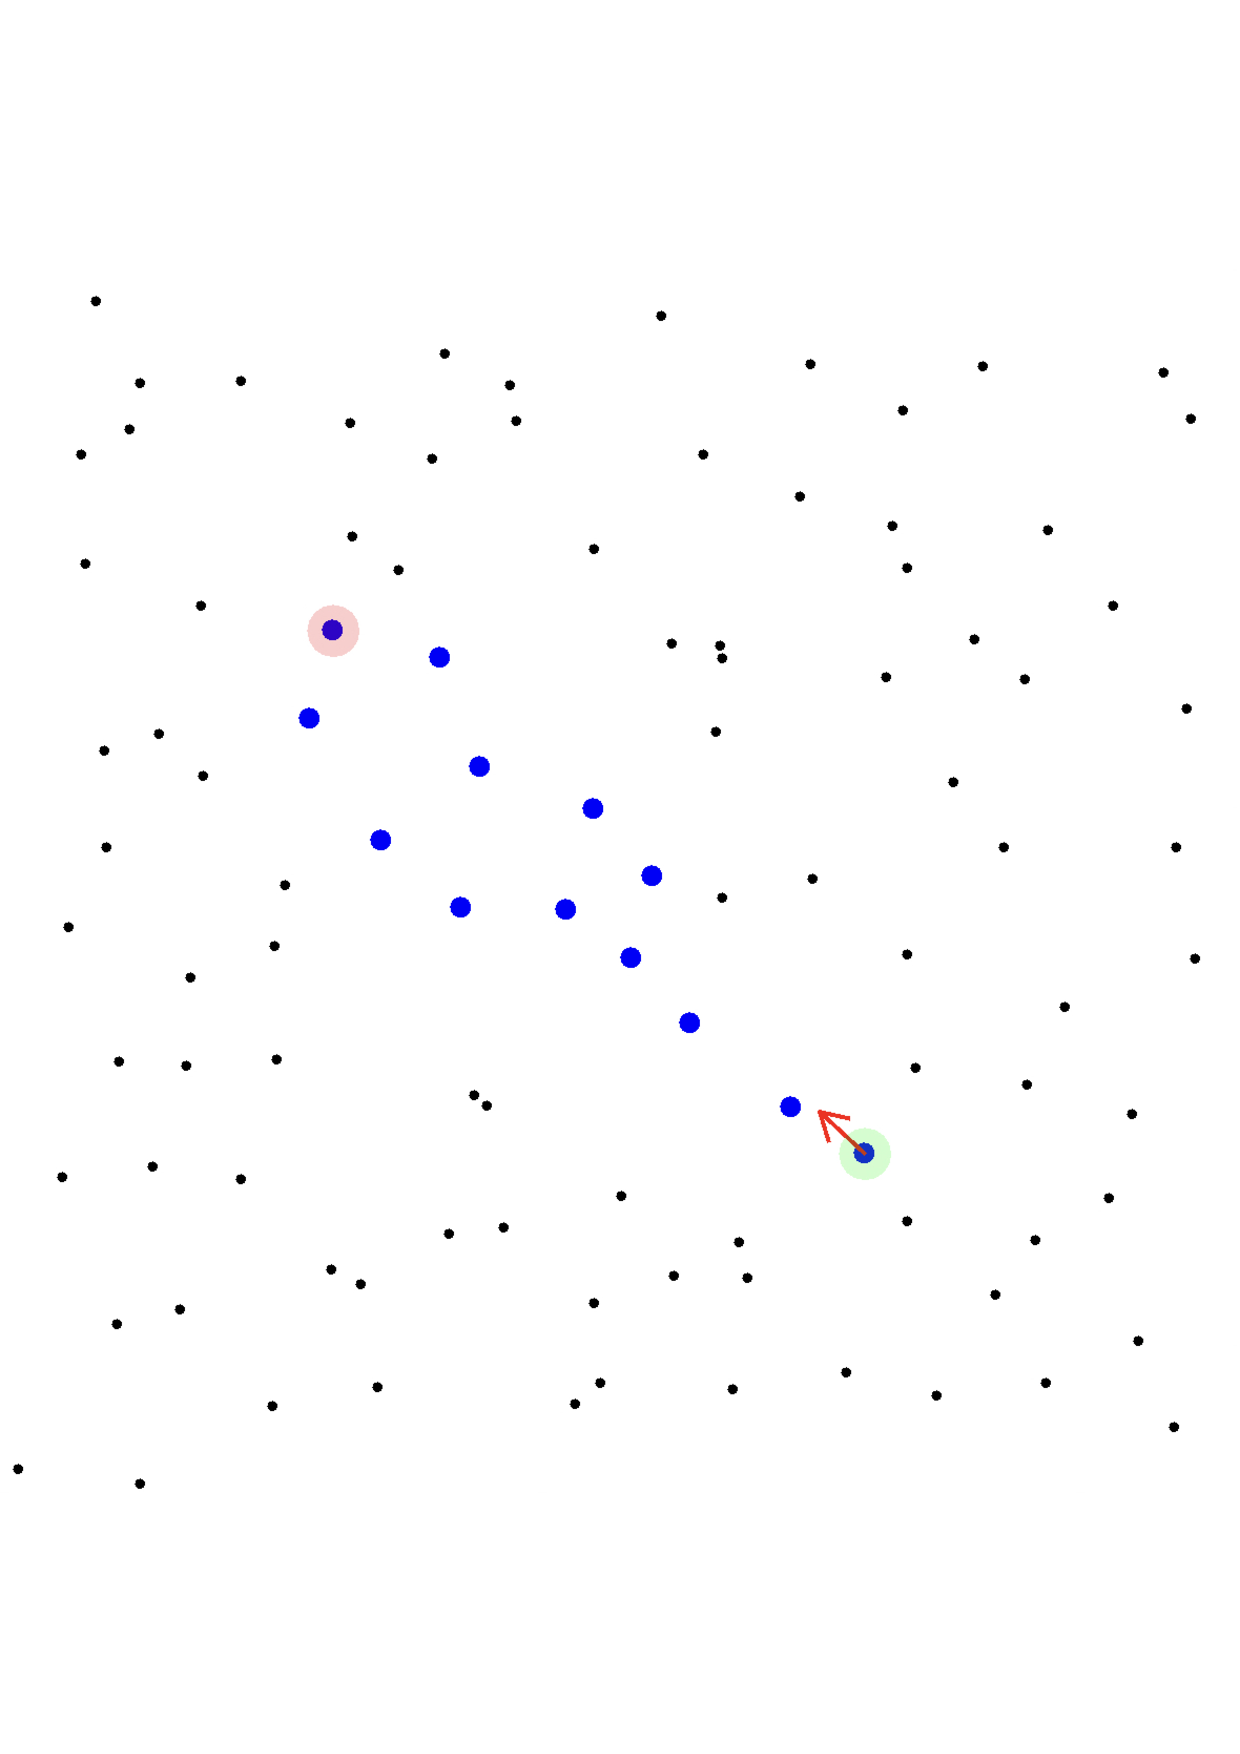
\includegraphics[width=.8\linewidth]{figures/track.pdf}
    \caption{Simulazione dell'esperimento in \cref{lst:trackck}.
    Il dispositivo target è evidenziato in rosso, mentre la destinazione in verde.
    I nodi che compongono il canale di comunicazione sono colorati in blu.
    La destinazione segue il target sfruttando le informazioni propagate lungo il canale.
    }
    \label{fig:track-simulation}
\end{figure}

\newpage
\section{Dinamica di uno stormo}
\label{sec:flock}

\paragraph{Obiettivo} Simulare la dinamica di uno stormo.

Ciascun dispositivo calcola la propria velocità in funzione della direzione iniziale, della distanza dai nodi vicini e delle loro rispettive direzioni di movimento.
%
La direzione iniziale è determinata dal ruolo del nodo: se il dispositivo è un "leader", viene orientato verso l'origine del sistema di coordinate; in caso contrario, la direzione iniziale è nulla.
%
La velocità, che evolve dinamicamente nel tempo, viene aggiornata secondo logiche di repulsione, coesione e allineamento, in base alla distanza dai vicini.
%
La direzione risultante è data dalla somma ponderata dei contributi di ciascun vicino, insieme alla direzione iniziale.

\paragraph{Codice originale} La funzione \texttt{flock} (\Cref{lst:flock}) richiede in ingresso la direzione di partenza (\texttt{dir}) del dispositivo.
%
\lstinputlisting[
    language=Lisp,
    label={lst:flock},
    caption={Codice della funzione \texttt{flock} in Proto.}
]{listings/proto/flock.proto}
%
L'evoluzione temporale della velocità dei nodi è gestita dall'istruzione \texttt{(rep v (tup 0 0 0) \dots)}.
%
Ad ogni round, viene determinato il vettore risultante \texttt{d} come somma dei contributi di repulsione, coesione e allineamento, provenienti dai dispositivi nel vicinato.
%
I contributi dei vicini vengono calcolati e aggregati tramite la funzione \texttt{int-hood \dots}, seguendo queste regole:
\begin{itemize}
    \item Se la distanza da un vicino è inferiore a $5$ unità (\texttt{(if (< (nbr-range) 5) \dots)}), il contributo è un vettore che allontana dall'entità vicina. Si calcola come il versore diretto verso il vicino, moltiplicato per \(-1\) (\texttt{(* -1 (normalize (nbr-vec)))}).
    \item Se la distanza è superiore a $10$ unità (\texttt{(if (> (nbr-range) 10) \dots)}), si esercita un'attrazione. Il contributo è il versore orientato verso il vicino, scalato di $0.2$ (\texttt{* 0.2 (normalize (nbr-vec))}).
    \item Se la distanza è compresa tra $5$ e $10$ unità, l'entità si allinea alla direzione attuale del vicino. Il contributo è dato dalla velocità attuale del vicino normalizzata (\texttt{normalize (nbr v)}).
\end{itemize}
%
Infine, la nuova velocità è determinata tramite l’espressione \texttt{(+ dir (mux (> (vdot d d) 0) d v))}: questa istruzione somma la direzione iniziale \texttt{dir} al vettore risultante \texttt{d} se la sua norma è positiva; in caso contrario, mantiene la velocità precedente \texttt{v}.
\paragraph{Trasposizione in Collektive} La traduzione in Collektive è riportata in \cref{lst:flockck}.

L’evoluzione della velocità dei nodi è gestita tramite l’operatore \texttt{share} (\Cref{lst:collektiveshare}) , poiché la dinamica dipende sia dallo stato dei vicini sia dallo stato calcolato nel round precedente.

La necessità di una migliore approssimazione contigua del campo ha portato all’introduzione delle funzioni ausiliarie \texttt{sumWeightedNeighbors} e \texttt{spatialWeight} (\Cref{lst:inthoodck}), che calcolano rispettivamente la somma pesata dei contributi dei vicini e il peso attribuito a ciascun nodo adiacente.
%
Il peso assegnato si ottiene dividendo l'area del cerchio, il cui raggio è pari a quello di comunicazione, per il numero di dispositivi presenti nel vicinato.

La simulazione dell’esperimento (\Cref{fig:flock-simulation}) mostra i nodi coordinatori evidenziati in rosso. 
%
Si osserva come i dispositivi si organizzino spontaneamente in tre stormi, ciascuno dei quali si dirige verso l’origine grazie alla presenza di un numero sufficiente di leader che guidano il movimento collettivo.
\newpage
\lstinputlisting[
    language=Kotlin,
    label={lst:flockck},
    caption={Trasposizione della funzione \texttt{flock} (\ref{lst:flock}) in Collektive.}
]{listings/collektive/Flock.kt}

\lstinputlisting[
    language=Kotlin,
    label={lst:inthoodck},
    caption={Supporto per la simulazione di \texttt{int-hood} in Collektive.}
    ]{listings/collektive/IntHood.kt}

\begin{figure}
    \centering
    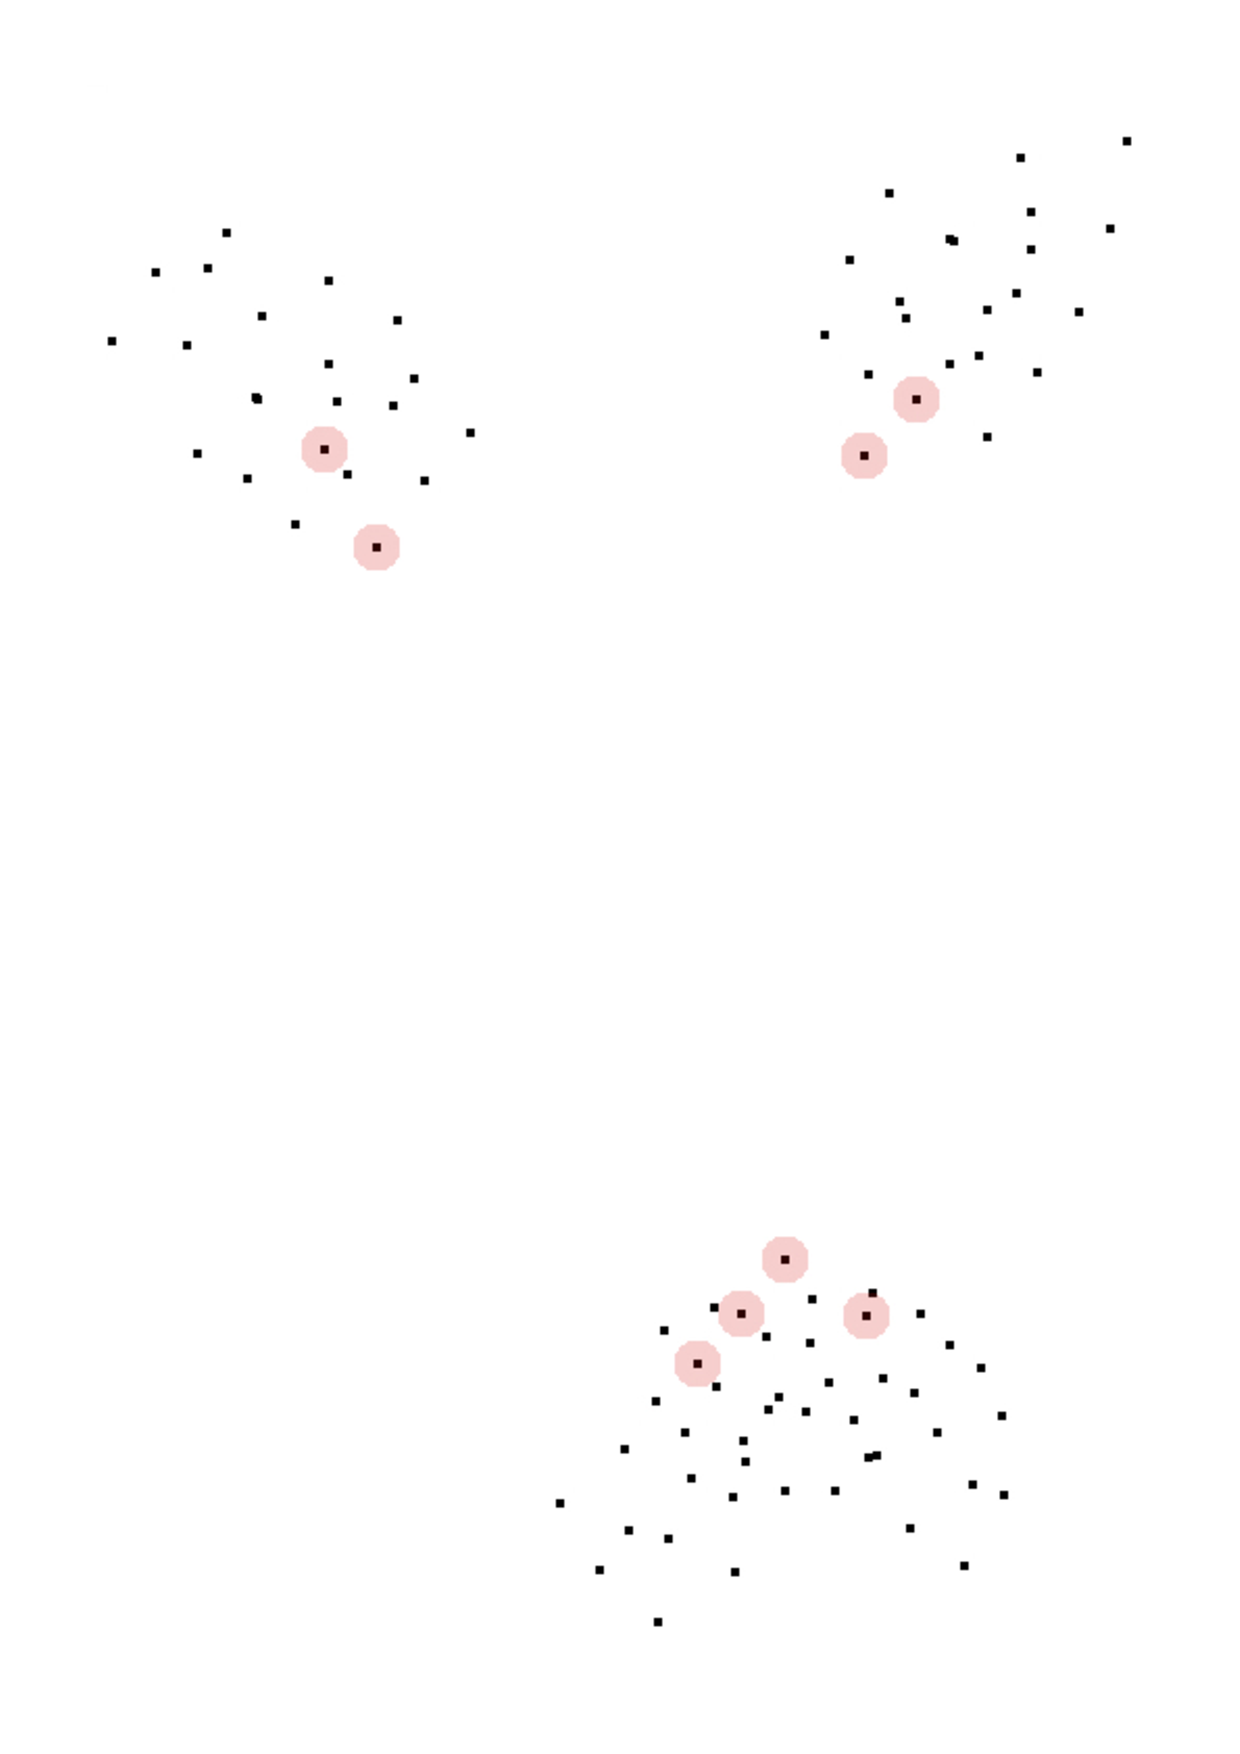
\includegraphics[width=.8\linewidth]{figures/flock.pdf}
    \caption{Simulazione dell’esperimento in \cref{lst:flockck}.
    I dispositivi leader sono colorati in rosso, mentre gli altri sono colorati in blu.
    Si osserva come i nodi si organizzino spontaneamente in tre stormi, ciascuno dei quali si dirige verso l’origine grazie alla presenza di un numero sufficiente di leader che guidano il movimento collettivo.
    }
    \label{fig:flock-simulation}
\end{figure}

\newpage
